\chapter{Introduction}
\label{ch.intro}

% Context
% - Historical background moore:1965
% -- Frequency barrier
	For some years now, it was common to increase the frequency of processors
	to improve their processing power.
	However, as a side effect, the temperature rise was much higher than the
	performance, making this practice prohibitive.
	Alternatively, the constant improvement of semiconductor technology helped
	to mitigate the impact of this problem, permitting the industry to build
	more powerful processors with the same frequency.
	Therefore, knowing the frequency barrier and the imminent end of Moore's Law~\cite{moore:1965},
	the academy and the industry began to research and invest in alternatives
	to keep increasing the processing power of computer systems.

% -- Improves architectural parts
	Such researches have led to a wide diversity of trade-offs in modern architectures.
	For instance, different types of instruction sets, instruction parallelism,
	out-of-order processing techniques, detour prediction techniques, and various
	memory hierarchies were some of the key techniques proposed to improve the
	performance of a single core.
	Then, the performance of computer systems has been improved even further by
	increasing the number of processing cores in a single die.
	These architectures, called \textit{multicores}, allowed the continuous
	rise of the computing performance.

	In some point, with reduction of transistors and the number of cores inside
	a multiprocessor began to scale, these architectures must be called \manycores.
	Notwithstanding, the line between \textit{multicores} and \manycores is very tenuous.
	Some researchers stipulate that the difference lies when losing a core
	does not impact the rest of the system.

	\begin{figure}[h]
		\centering
		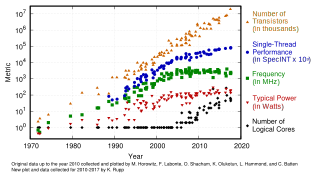
\includegraphics[width=.85\textwidth]{images/42-years-processor-trend.pdf}

		\caption{
			42 years of Multiprocessor Trend Data~\cite{url:microprocessor-trend-data}.
		}\par
		\label{fig.microprocessor-data}
	\end{figure}

% - From multicore to manycores

	However, Figure \ref{fig.microprocessor-data} shows that, in recent years,
	the energy consumption of parallel processors has become as crucial as their
	processing power, which is usually measured by the number of \flops.
	At this point, with the popularization of embedded systems as well as the aim
	to reach the \exascale (10$^{18}$ \flops), a new class of parallel processors,
	named \textit{lightweight} \manycores, emerged to provide high parallelism
	with low-power consumption.

% FROM FUNDAMENTATION
% {
	% With the enhancement of technologies and the reduction of transistors,
	% the number of cores inside a multiprocessor began to scale.
	% Until at some point, these architectures must be called \manycores.
	% However, the line between multi-cores and \manycores is very tenuous.
	% Some researchers stipulate that the difference lies when losing a core
	% does not impact the rest of the system.
	% In this way, \manycores are as multi-cores with tens, hundreds, or even
	% thousands of cores, presenting the most diverse architectural properties.
	% For example, there are \uma/\numa multiprocessors with \simd present on
	% \gpus, and \numa multiprocessors with \mimd as \mppa presented in Section \ref{sec.multiprocessor-hw}.

	% A promising class of \manycores began to emerge, aiming the energy barrier
	% that we will face in the future.
	% \textit{Lightweight Manycores} stand out for their performance compared
	% to their energy consumption.
	% However, due to its particular characteristics, several problems of
	% programmability, portability, and performance are still open.
% }

% - Manycores characteristics
	The \textit{lightweight} \manycores
		(i) integrate thousands of low-power cores in a single die organized in clusters;
		(ii) are designed to cope with \mimd workloads;
		(iii) rely on a high-bandwidth \noc for fast and reliable message-passing communication;
		(iv) present constrained memory systems; and
		(v) frequently feature a heterogeneous configuration.
	Some industry-successful examples of \textit{lightweight} \manycores are
	the \mppa~\cite{DeDinechin2013-1};
	the \epiphany~\cite{olofsson2014}; and
	the \taihulight~\cite{zheng2015}.

% Motivation
% - Difficults from Manycores
	Jointly with further performance scalability and energy efficiency, manycores brought a new
	set of challenges in software development coming from their architectural particularities.
	Precisely, these particularities introduce the following difficulties:
	\begin{itemize}
		\item \textbf{Hybrid programming model:} due to the parallel and distributed nature of
			the architecture, engineers are frequently required to adopt a message-passing
			programming model to deal with the presence of rich \nocs~\cite{kelly2013} that
			interconnects clusters and a shared-memory model inside the cluster.
		\item \textbf{Missing hardware support for cache coherency:} to reduce power consumption,
			theses processors do not feature cache coherency, which in turn forces programmers to
			handle it explicitly in software level and frequently calls out for a redesign in their
			applications~\cite{francesquini2015};
		\item \textbf{Constrained memory system:} the frequent presence of multiple physical
			address spaces and small local memories require data tiling and prefetching to be
			handled by the software~\cite{Castro2016};
		\item \textbf{Heterogeneous configuration:} the different programmable components on
			\textit{lightweight} \manycores turns the actual deployment of applications in a
			complex task~\cite{barbalace2015}.
	\end{itemize}

% - Why is development on manycores difficult?
	Part of these challenges derives from existing \oses and runtimes.
	On the one hand, the complicated portability and scalability of traditional \oses with a
	monolithic kernels, which were designed to homogeneous hardwares, is leading to the development
	of new \oses from scratch~\cite{Baumann2009, kluge2014, nightingale2009, rhoden2011}.
	On the other hand, existing runtimes only partially address some of the programmability issues
	of \textit{lightweight} \manycores, making the process of developing, porting, and maintaining
	applications a challenging task.

% Challenges and Problem Definition
% - How are OSs essential in this context?

% - Why these problems exist? (Because the existing OSes does not handle architecture particularities)
% - These particularities prevent common OSes that easy portated without a complex redesign. And existing OSes does not account some architectural points.

% Goals and Contributions
% - Redesign from scratch around all their tight architectural constraints.
% - Focus on addressing first-order programmability challenges
% - Introducing generic and flexible HAL for lightweight manycores
	% Nexte contexto, o doutorando e coorientador deste trabalho, Pedro H. Penna, mirando a maior programabilidade e portabilidade para lightweight manycores, propoe que sistemas operacionais para essa nova geração de processadores deve ser reprojetada do zero baseando-se em todas as suas restrições arquiteturais.
	% Sua proposta envolve um sistema operacional completo distribuido baseado em uma arquitetura multikernel~\cite{multikernel}.
	% Para isso, baseados em resultados de serviços experimentais desenvolvidos encimado do mppa256~\cite{rmem}, a pesquisa começou buscando resolver os primeiros desafios que surgiram.
	% Especificamente, foi introduzido uma \hal genérica e flexivel para lightweight manycores que lidam com os problemas chaves encontrados no desenvolvimento para esses processadores.
	% Em seguida, a pesquisa seguirá em desenvolver um microkernel para prover os mecanismos básicos para desenvolvimento de um OS completo sobre ele.
	% Por fim, o desenvolvimento de serviços do multikernel serão alcançados.

	We believe that \oses for the next-generation of \textit{lightweight} \manycores must be
	redesigned from scratch to cope with their tight architectural constraints.
	Based on this idea, a new fully-featured distributed \os based on a \multikernel approach~\cite{Baumann2009}
	is being proposed~\cite{penna2017-1,penna2017-2,penna2019}.
	Nanvix features a generic and flexible \hal for \textit{lightweight} \manycores that
	addresses the key issues encountered in the development for these processors.
	On top of the Nanvix \hal, we are simultaneously designing and implementing a \microkernel
	that provides bare bones system abstractions for each cluster.

	In this monograph, we intend to propose a Inter-Cluster Communication Module to the Nanvix \hal
	and port it to the \mppa manycore processor~\cite{DeDinechin2013-1}.
	Using this module, we also pretend design Inter-Cluster Communication Services to the Nanvix \microkernel.
	This work will be done in collaboration with Pedro H. Penna, who is a Ph.D. student at the
	University of Grenoble Alpes, the main developer of Nanvix and the co-advisor of this work.
	Then, we will analyze the performance of the proposed implementation using specific micro-benchmarks.

\section{Objectives}

	This will be written last.
%    Assist to research and develop \hal for \textit{lightweight} manycores.

\subsection{General Objective}

	This will be written last.
%    On the basis of the foregoing, the following general objective and the specific objectives of this project.

\subsection{Specific Objectives}
   \begin{itemize}
		\item This will be written last.
    %    \item Present and discuss hal \textit{lightweight} manycores.
    %    \item Design and develop the Inter-cluster communication module.
    %    \item Assist in the development and improvement of other modules.
    %    \item Perform a performance analysis of the proposed \hal for the \mppa.
   \end{itemize}

\section{Organization Of The Work}

	This will be written last.